\section{Implementation} \label{sec:implementation}
\subsection{Neural Network Algorithm Implementation}

\begin{frame}
\begin{tikzpicture}[node distance=2cm]
\node (start) [startstop] {Start};
\node (in1) [io, below of=start] {Input};
\node (pro1) [process, below of=in1] {Process 1};
\node (dec1) [decision, below of=pro1] {Decision 1};
\node (dec1) [decision, below of=pro1, yshift=-0.5cm] {Decision 1};
\node (pro2a) [process, below of=dec1, yshift=-0.5cm] {Process 2a};
\node (pro2b) [process, right of=dec1, xshift=2cm] {Process 2b};
\node (out1) [io, below of=pro2a] {Output};
\node (stop) [startstop, below of=out1] {Stop};
\draw [arrow] (start) -- (in1);
\draw [arrow] (in1) -- (pro1);
\draw [arrow] (pro1) -- (dec1);
\draw [arrow] (dec1) -- (pro2a);
\draw [arrow] (dec1) -- (pro2b);
\draw [arrow] (dec1) -- node[anchor=east] {yes} (pro2a);
\draw [arrow] (dec1) -- node[anchor=south] {no} (pro2b);
\draw [arrow] (pro2b) -- (pro1);
\draw [arrow] (pro2a) -- (out1);
\draw [arrow] (out1) -- (stop);
\draw [arrow] (pro2b) |- (pro1);
\end{tikzpicture}
\end{frame}

\begin{frame}
\smartdiagram[priority descriptive diagram]{
  Develop a document structure,
  Choose a document class,
  Select suitable packages,
  Setup the document preamble,
  Write your document,
  Finetune the layout}
\end{frame}

\begin{frame}
\begin{center}
\smartdiagram[bubble diagram]{
Build a program,1,2,3,Modify~/\\ Add,5, 6,7
}
\end{center}
\end{frame}

\begin{frame}
\smartdiagramset{set color list={blue!40!yellow, blue!40!orange, blue!40!red, blue!40!purple, blue!40!gray}}
\tikzset{priority arrow/.append style={rotate=180,anchor=0,xshift=30,}}
\smartdiagram[priority descriptive diagram]{yellow, orange, red, purple, blue}
\end{frame}

\begin{frame}
\begin{columns}[T] % align columns
\begin{column}{.48\textwidth}
\color{red}\rule{\linewidth}{4pt}
\smartdiagramset{set color list={blue!40!yellow, blue!40!orange, blue!40!red, blue!40!purple, blue!40!gray}}
\tikzset{priority arrow/.append style={rotate=180,anchor=0,xshift=30,}}
\smartdiagram[priority descriptive diagram]{yellow, orange, red, purple, blue}
\end{column}%
\hfill%
\begin{column}{.48\textwidth}
\color{blue}\rule{\linewidth}{4pt}

\smartdiagramset{set color list={blue!40!yellow, blue!40!orange, blue!40!red, blue!40!purple, blue!40!gray}}
\tikzset{priority arrow/.append style={rotate=180,anchor=0,xshift=30,}}
\smartdiagram[priority descriptive diagram]{yellow, orange, red, purple, blue}
\end{column}%
\end{columns}
\end{frame}

\begin{frame}{The minipage environment}
\begin{minipage}{0.47\textwidth}
    \begin{itemize}
        \item First item
        \item Second item
        \item Third item
    \end{itemize}
\end{minipage}
\resizebox{5.0cm}{!}{%
    \smartdiagramset{set color list={blue!40!yellow, blue!40!orange, blue!40!red, blue!40!purple, blue!40!gray}}
\tikzset{priority arrow/.append style={rotate=180,anchor=0,xshift=30,}}
\smartdiagram[priority descriptive diagram]{yellow, orange, red, purple, blue}
}%
\end{frame}

% \begin{frame}
%  \centering
%  \begin{figure}
%    \only<1-3>{
%        \begin{subfigure}[b]{0.3\textwidth}
%          \caption{Free Positioning}
%                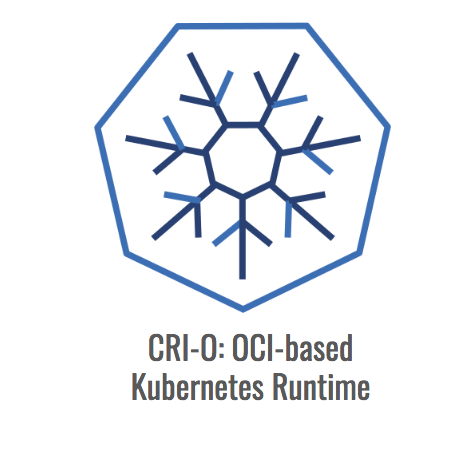
\includegraphics[width=\textwidth,height=\textwidth]{./png/crio}
%                \label{fig:guided}
%                \setcounter{subfigure}{0}% Reset subfigure counter
%        \end{subfigure}\hfill
%        }
%    \only<2-3>{
%        ~ %add desired spacing between images, e. g. ~, \quad, \qquad etc.
%          %(or a blank line to force the subfigure onto a new line)
%        \begin{subfigure}[b]{0.3\textwidth}
%        \setcounter{subfigure}{1}% Reset subfigure counter
%          \caption{Neural Network}
%                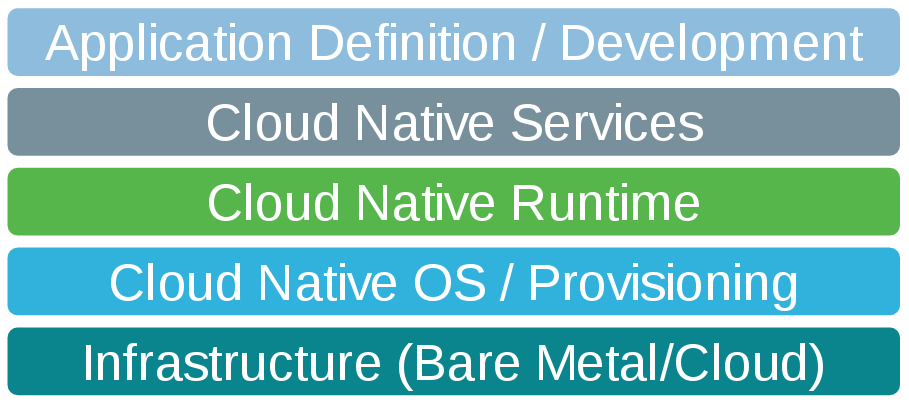
\includegraphics[width=\textwidth,height=\textwidth]{./png/cri}
%                \label{fig:free}
%        \setcounter{subfigure}{0}% Reset subfigure counter
%        \end{subfigure}\hfill
%        }
%    \only<3-3>{
%        ~ %add desired spacing between images, e. g. ~, \quad, \qquad etc.
%          %(or a blank line to force the subfigure onto a new line)
%        \begin{subfigure}[b]{0.3\textwidth}
%            \setcounter{subfigure}{2}% Reset subfigure counter
%          \caption{Matlab Output}
%                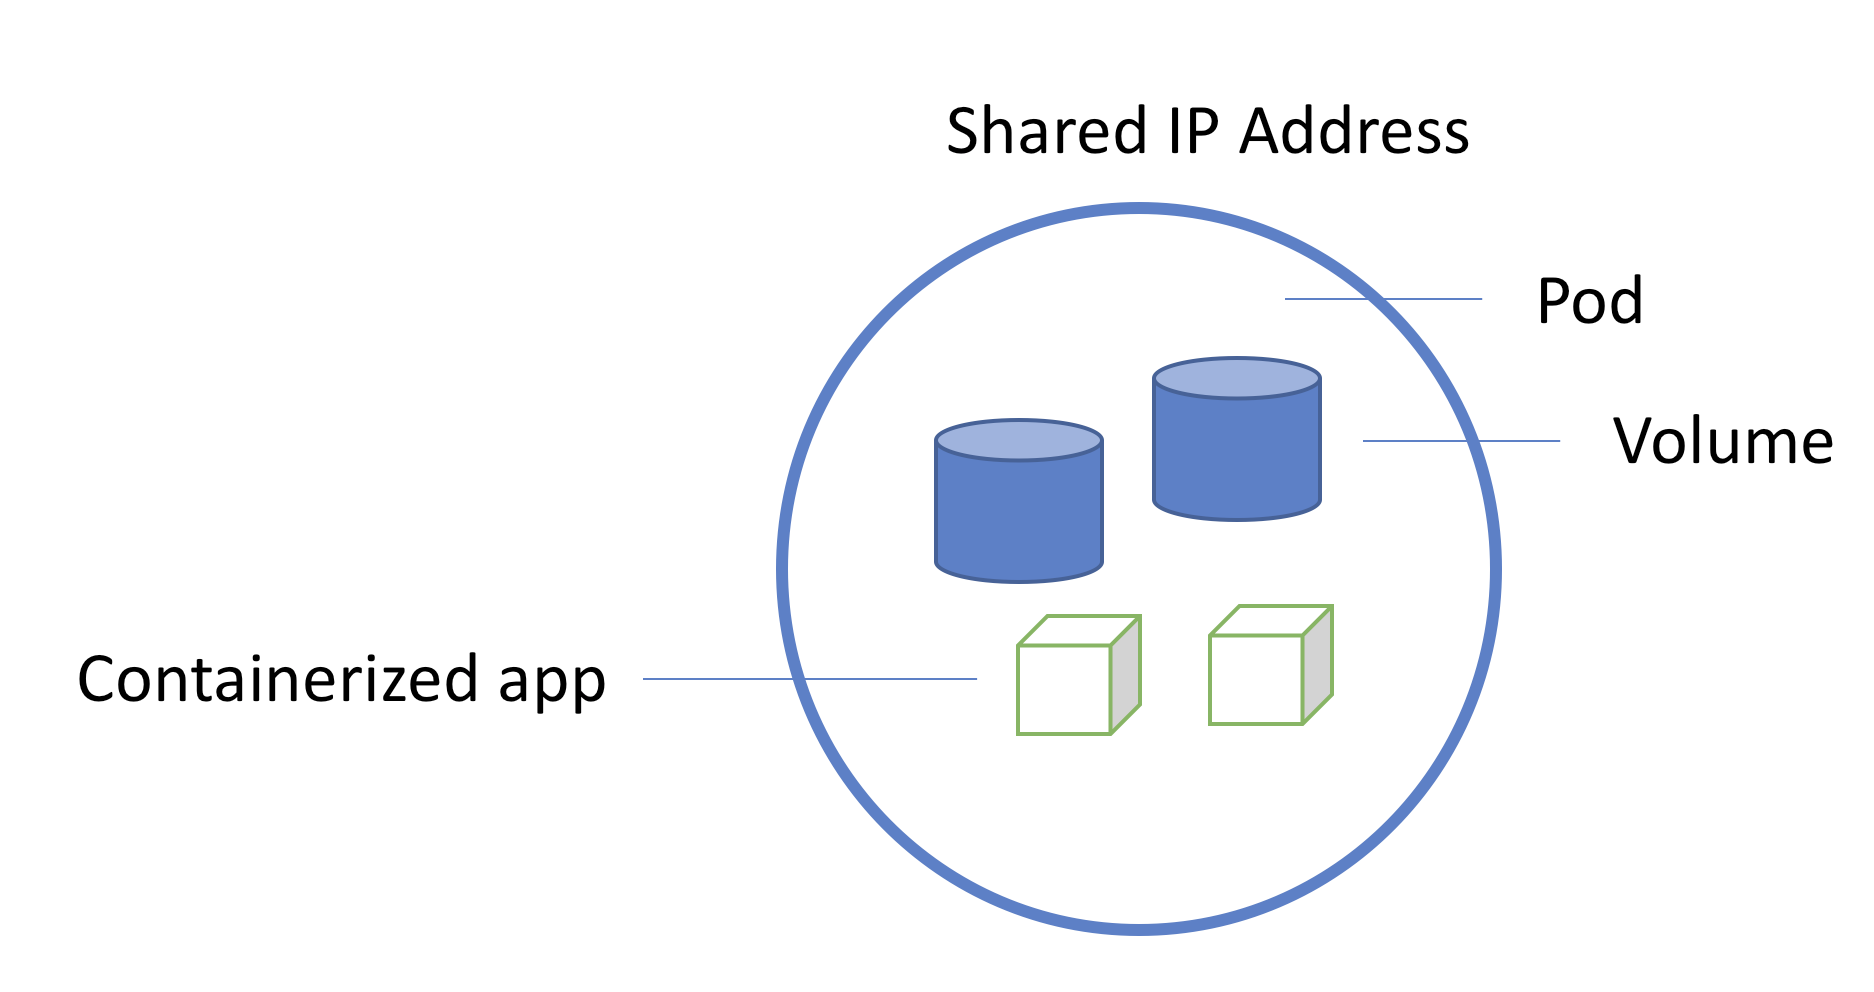
\includegraphics[width=\textwidth,height=\textwidth]{./png/pod}
%                \label{fig:multiple}
%        \end{subfigure}%
%        }
%        \caption{Different wireless charging approaches~\label{fig:animals}}
%  \end{figure}
%  \begin{itemize}[<+->]
%      \item<1-| alert@1> Free positioning charging based on Inductive coupling~\cite{wireless}.
%      \item<2-| alert@2> Based on RLoad and Frequency Input and Output~\cite{wireless}. %\ref{fig:free}
%      \item<3-| alert@3> Simulation of Matlab Output based on RLoad as an Input~\cite{wireless}. %   \ref{fig:multiple}
%  \end{itemize} 
%\end{frame}
